\newpage
\section{Overview}
\label{sec::overview}
Anya can be thought of as a particular implementation of A{*} search. 
It uses the same principles as that algorithm: there is an open
and a closed list, there is an admissible heuristic function 
(in this case, Euclidean distance) and the search proceeds by generating
and expanding nodes in the order of minimum $f$-value.
What differentiates Anya from other algorithms is (i) how we define 
search nodes; (ii) how we evaluate search nodes and; 
(iii) how we identify the successors of each search node.

Like other search algorithms Anya requires two discrete points from the grid:
a start location and a target location.
To find a path a typical search algorithm will generate and expand single
points from the grid until the goal is reached or the open list is exhausted.
Anya differs from these methods because it does not consider single points.
Instead, Anya generates and expands an \emph{entire set} of points at one time.
Each set is a contiguous interval of traversable points -- all drawn from a 
single row of the grid.
Expanding a node means projecting an interval along the current row
of the grid or from the current row to an adjacent row. Evaluating a node means 
selecting from the interval a single representative point which is used
to compute an $f$-value for the entire set.
Example~\ref{ex::anya_example} illustrates how Anya proceeds during pathfinding search.

\begin{figure}[hb]
\center
\begin{minipage}{0.45\columnwidth}
\center
		   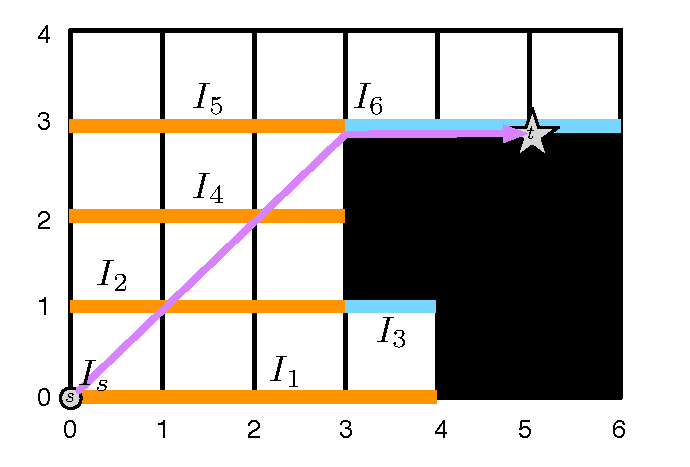
\includegraphics[width=\columnwidth]
			{images/anya_example.pdf}
	\vspace{-3pt}
\end{minipage}
\begin{minipage}{0.45\columnwidth}
\center
		   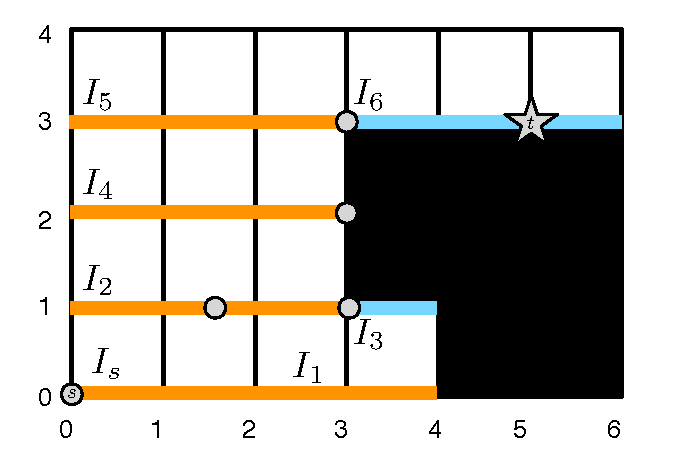
\includegraphics[width=\columnwidth]
			{images/anya_example_b.pdf}
	\vspace{-3pt}
\end{minipage}
\caption{
\small
\textbf{(Left)} Searching with Anya. The starting and target locations are designated $s$ and $t$.
We show six intervals generated by the search process. Each interval is highlighted in orange. 
The optimal any-angle path is highlighted in purple. 
\textbf{(Right)} We show the representative points computed for each interval. The representative
points for $I_s$ and $I_1$ are almost the same: the starting point $s = (0, 0)$ and the point $p = (0+\epsilon, 0)$
where $\epsilon$ is a very small number. We do not attempt to distinguish between them pictorially.
}
\label{fig::anya_example}
\end{figure}

\begin{example}
\label{ex::anya_example}
Consider Figure~\ref{fig::anya_example} (Left). 
We want to find a path from the starting location $s$ to the target location $t$.
To represent the start node we construct a single point interval $I_s = [s]$. 
Expanding $I_s$ yields three contiguous intervals: $I_1$, $I_2$ and $I_3$.
Of these only $I_2$ is not sterile and expanding it yields another interval, $I_4$.
Continuing the process and expanding $I_4$ yields intervals $I_5$ and $I_6$.
The latter contains the goal and expanding it terminates the search.
The optimal any-angle path from $s$ to $t$ is a taut sequence of 
straight lines that starts with $s$, ends with $t$ and passes through the intervals
$I_1$, $I_2$, $I_4$ and $I_6$. Taut simply means that if we ``pull'' on the endpoints
of this path we cannot make it any shorter.
Recall that each time A* search generates a successor it needs to compute an $f$-value
to prioritise its expansion. We achieve this by selecting from each interval a 
single representative point. To ensure that the search process always returns
an optimal path we always choose the point with minimum $f$-value 
from among all points in the set. 
Figure~\ref{fig::anya_example}~(Right) shows the representative points
for every interval in this example.
Notice that the optimal path is not required to pass through the representative points.

\end{example} 

%The representative points used to evaluate each interval in the example 
%are shown in Figure~\ref{fig::anya_example} (Right). 
In the next sections we will discuss (i) how to construct intervals;
(ii) how to represent search nodes; (iii) how to generate successors; 
(iv) how to select representative points.
